\documentclass{article}
\usepackage{fullpage}
\usepackage{amsfonts}
\usepackage{amssymb}
\usepackage{amsmath}
\usepackage{hyperref}
\usepackage{graphicx}% Include figure files
\usepackage{epstopdf}
\usepackage{subfig}
\usepackage{appendix}
%\usepackage{setspace}\doublespace
\author{Guojun Zhu}
\title{My Daily Note}
\newcommand{\vk}{\ensuremath{\mathbf{k}}}
\newcommand{\vK}{\ensuremath{\mathbf{K}}}
\providecommand{\vr}{\ensuremath{\mathbf{r}}}
%\newcommand{\vec}[1]{\ensuremath{\mathbf{#1}}}

\newcommand{\gk}{\ensuremath{{g}(\mathbf{k})}}

\newcommand{\vp}{\ensuremath{\mathbf{p}}}
\newcommand{\gp}{\ensuremath{{g}(\mathbf{p})}}

\newcommand{\vq}{\ensuremath{\mathbf{q}}}

\newcommand{\Fo}{\ensuremath{\mathbf{F_0}}}


\newcommand{\E}{\ensuremath{\mathbf{E}}}
\newcommand{\A}{\ensuremath{\mathbf{A}}}
\newcommand{\J}{\ensuremath{\mathcal{J}}}

\newcommand{\ket}[1]{\ensuremath{\left|#1\right>}}
\newcommand{\bra}[1]{\ensuremath{\left<#1\right|}}

\newcommand{\twoe}{\ensuremath{2\epsilon_\vk-\E_1}}

\newcommand{\nth}[1]{\ensuremath{\frac{1}{#1}}}

\newcommand{\br}[1]{\ensuremath{\left(#1\right)}}
\newcommand{\mbr}[1]{\ensuremath{\left[#1\right]}}
\newcommand{\bbr}[1]{\ensuremath{\left\{#1\right\}}}


\newcommand{\tk}{\ensuremath{\tilde{k}}}

\newcommand{\kp}{\ensuremath{\ket{\Psi}}}

\newcommand{\av}[1]{\ensuremath{\bigl<{#1}\bigr>}}
\newcommand{\avs}[3] {\av{#1{\lvert{#2}\rvert}#3}}
\newcommand{\avv}[2][\nu] {\avs{#1}{#2}{#1}}
\newcommand{\avt}[2]{\av{{#1}|{#2}}}
\newcommand{\avtu}[1]{\av{T_\tau#1}}

\newcommand{\Bop}{\ensuremath{\mathbf{B_0^+}}}
\newcommand{\Bmp}{\ensuremath{\mathbf{B_m^+}}}
\newcommand{\Bnp}{\ensuremath{\mathbf{B_n^+}}}
\newcommand{\Bo}{\ensuremath{\mathbf{B_0}}}
\newcommand{\Bopn}{\ensuremath{\mathbf{{B_0^+}^n}}}
\newcommand{\Bon}{\ensuremath{\mathbf{{B_0}^n}}}


\newcommand{\zmatrix}{\ensuremath{\br{\begin{smallmatrix}0&0\\0&0\end{smallmatrix}}}}
\newcommand{\fmtrx}[4]{\ensuremath{\br{\begin{smallmatrix}#1&#2\\#3&#4\end{smallmatrix}}}}
\newcommand{\smtrx}[6]{\ensuremath{\br{\begin{smallmatrix}#1&#2\\#3&#4\\#5&#6\end{smallmatrix}}}}

\newcommand{\vz}{\ensuremath{v^{\beta\alpha}_{\vk,\vk}}}


\providecommand{\abs}[1]{\ensuremath{\lvert{#1}\rvert}}

\newcommand{\sg}[1][1]{\ensuremath{\sigma_\frac{#1}{2}}}

\newcommand{\rhof}{\ensuremath{\rho(\ef)}}
\newcommand{\omt}{\ensuremath{\tilde{\Omega}}}
\newcommand{\cht}{\ensuremath{\tilde{\chi_0}}}
\newcommand{\Atl}{\ensuremath{\abs{A}^{2l}}}
\newcommand{\ef}{\ensuremath{\epsilon_F}}

\newcommand{\lca}{\ensuremath{\ln\br{1+\frac{\cht}{\alpha}}}}

\newcommand{\com}[2]{\ensuremath{\mbr{#1,#2}}}
\newcommand{\D}{\ensuremath{\mathit{D}}}
\newcommand{\dg}{\ensuremath{\dagger}}
\newcommand{\nG}{\ensuremath{\hat{\mathcal{G}}^{-1}}}

\providecommand{\lvk}{\ensuremath{1/\vk_F}}
\providecommand{\hm}{\ensuremath{\frac{\hbar^2}}{2m}}
\providecommand{\pdiff}[2]{\ensuremath{\frac{\partial{#1}}{\partial{#2}}}}
\providecommand{\dpdiff}[2]{\ensuremath{\frac{\partial^2{#1}}{\partial{{#2}^2}}}}

\providecommand{\H}{\ensuremath{\mathcal{H}}}
\providecommand{\wt}[1]{\widetilde{#1}}

\providecommand{\eef}[1]{Eq. (\ref{#1})}

\providecommand{\sch}{{Schr\"{o}dinger }}

\providecommand{\sgn}{\ensuremath{\text{sgn}}}
\newcommand{\Arctg}{\ensuremath{\text{Arctg}}}

\providecommand{\comm}[1]{\textit{\scriptsize \uwave{(#1)}}}
\renewcommand{\emph}[1]{\textbf{#1}}
\begin{document}
%\maketitle

%\tableofcontents
\numberwithin{equation}{section}


%\section{}
%\subsection{Two-Body Density Matrix in Richardson Solution}
As pointed in \cite{Leggett}, the existing of eigenvalue in order of $N$ in the two-body density matrix of BCS solution is probably the most fundamental fact of the superfluid phenomenon.  In the traditional BCS ansatz, the order parameter $F_\vk=u_\vk v^*_\vk$ is this eigenvector with the eigenvalue of $N_0=\frac{\pi}4\Delta{}N(0)\Omega$, \cite[(5.4.32)]{Leggett}.  Therefore it is important to check the solution with Richardson approach \cite{CobosonBcsRich} about this quantity.  What we are looking for is only zero-central-momentum eigenfunction, 
\begin{equation}\label{eq:2bodyDensityMatrixDef}
\av{\beta_\vk^\dg\beta_{\vk'}^{}}=\av{a_\vk^\dg{}b_{-\vk}^\dg{}b_{-\vk'}^{}{}a_{\vk'}^{}}
\end{equation}
Here we mostly follow the original paper's notion, with some short-hand explained as following:
\begin{equation}
 B^\dg_i=B^\dg(R_i)
\end{equation}
\begin{equation}
 \avt{i}{\vk}=\avv{B_i^{}\beta^\dg_\vk}
\end{equation}
\begin{equation}
 \avt{i}{j}=\avv{B_i^{}B^\dg_j}=\sum_\vk \avt{i}{\vk} \avt{\vk}{j}
\end{equation}

In the Richardson solution, ground wave-function is $\ket{\Psi_n}=\prod_i^n{}B^\dg_i\ket{\nu}$. Here different $B^\dg_i\ket{\nu}$'s are neither orthogonal nor normalized. In fact, they have rather substantial overlap most of the time.   Two-body density matrix here is further complicated by the fact that many-body wave-function is affected by the \emph{composite} nature of those cobosons. Generally,  
\begin{equation}
\av{\beta_\vk^\dg\beta_{\vk'}^{}}=\frac{\avv[\Psi_n]{\beta_\vk^\dg\beta_{\vk'}^{}}}{\avt{\Psi_n}{\Psi_n}}
\end{equation}.   

\subsubsection{Two pairs}
We started with a two-pair state, $\ket{\Psi_2}=B^\dg_i{}B^\dg_j\ket{\nu}$. 

\begin{equation}\label{eq:tbdm2pair}
\begin{split}
 &\avv[\Psi_2]{\beta_\vk^\dg\beta_{\vk'}^{}}\\
=&\mbr{\br{\avt{i}{j}\avt{j}{\vk}\avt{\vk'}{j}+\avt{i}{j}\avt{j}{\vk}\avt{\vk'}{i}}+(i\leftrightarrow{}j)}\\
  &-2\mbr{\br{\avt{j}{\vk}\avt{i}{\vk}\avt{\vk}{i}\avt{\vk'}{j}+\avt{\vk'}{i}\avt{\vk'}{j}\avt{j}{\vk}\avt{i}{\vk'}}+(i\leftrightarrow{}j)}\\
&+4\avt{j}{\vk}\avt{i}{\vk}\avt{\vk'}{i}\avt{\vk'}{j}\delta_{\vk\vk'}
\end{split}
\end{equation}
Here the first four terms (fig. \ref{fig:tbdm2pair1},\ref{fig:tbdm2pair2}) are from the paring, while the next eight terms (fig. \ref{fig:tbdm2pair3}-\ref{fig:tbdm2pair6}) as well as the last term  (fig. \ref{fig:tbdm2pair7}) are due to the Pauli exclusion of \emph{composite} nature. They show the moth-eaten effect.
\begin{figure}[htb]
\centering
  \subfloat[][]{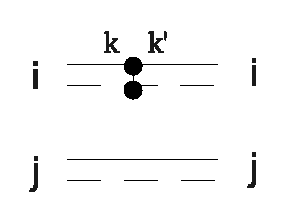
\includegraphics[width=0.2\textwidth]{image/tbdm2pair1.eps}\label{fig:tbdm2pair1}}\qquad
 \subfloat[][]{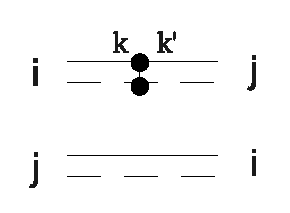
\includegraphics[width=0.2\textwidth]{image/tbdm2pair2.eps}\label{fig:tbdm2pair2}}\qquad
  \subfloat[][]{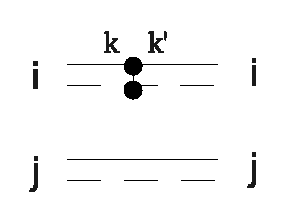
\includegraphics[width=0.2\textwidth]{image/tbdm2pair1.eps}\label{fig:tbdm2pair3}}\\
 \subfloat[][]{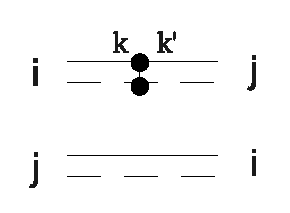
\includegraphics[width=0.2\textwidth]{image/tbdm2pair2.eps}\label{fig:tbdm2pair4}}\qquad
  \subfloat[][]{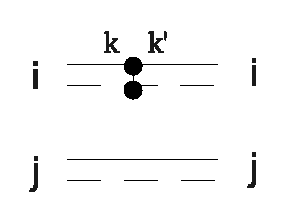
\includegraphics[width=0.2\textwidth]{image/tbdm2pair1.eps}\label{fig:tbdm2pair5}}\qquad
 \subfloat[][]{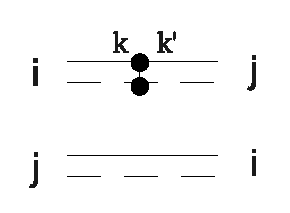
\includegraphics[width=0.2\textwidth]{image/tbdm2pair2.eps}\label{fig:tbdm2pair6}}\\
  \subfloat[][]{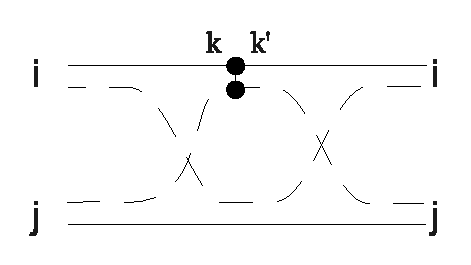
\includegraphics[width=0.3\textwidth]{image/tbdm2pair7.eps}\label{fig:tbdm2pair7}} 
\caption{Shiva diagram of two pairs }
\begin{description}
\item[\subref{fig:tbdm2pair1},\subref{fig:tbdm2pair2}] Signle pair without Pauli scattering.  There are also terms with $(i\leftrightarrow{j})$. First line of the above equation. 
\item[\subref{fig:tbdm2pair3},\subref{fig:tbdm2pair4},\subref{fig:tbdm2pair5},\subref{fig:tbdm2pair6}] Two-pair with Pauli scattering.  There are also terms with $(i\leftrightarrow{j})$. 
Second line of the equation. 
\item[\subref{fig:tbdm2pair7}] This coresponds the last term.  And there are the permutation of (i,j) as other terms.  
\end{description}
\end{figure}

The last term is especially interseting as this is two separate pieceses (fig.\ref{fig:shivaseparate}).  Normally, they do not exist, but here they do show up because we need pair of $\vk$,$\vk'$ .  
\begin{figure}[htb]\centering
 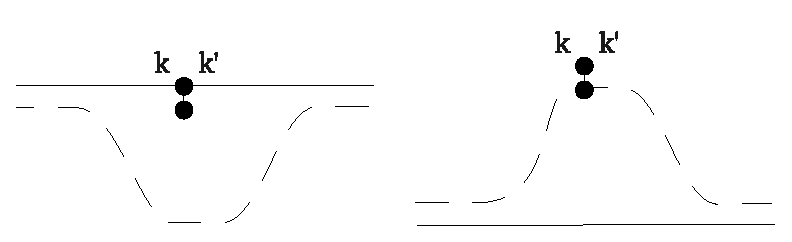
\includegraphics[width=0.3\textwidth]{image/shivaSeparate.eps}
\caption{Two separate connection parts of the last term of \eqref{eq:tbdm2pair}\label{fig:shivaseparate}}\centering
\end{figure}
And the normalization factor:
\begin{equation}
 {\avt{\Psi_2}{\Psi_2}}=\av{B^{}_j{}B^{}_i{}B^\dg_i{}B^\dg_j}=\avt{i}{i}\avt{j}{j}+\abs{\avt{i}{j}}^2-2\sum_\vk\avt{j}{\vk}\avt{i}{\vk}\avt{\vk}{i}\avt{\vk}{j}
\end{equation}

\subsubsection{Three pairs}
For a three-pair state $\ket{\Psi_3}=B^\dg_i{}B^\dg_j{}B^\dg_m\ket{\nu}$. 
we have 
\begin{equation}
\begin{split}
 \bra{\Psi_3}\beta^\dg_\vk=&\bra{\nu}B_m{}B_j{}B_i\beta^\dg_\vk\\
=&-2\avt{j}{\vk}\avt{m}{\vk}\bra{\nu}\beta_\vk{}B_i-2\avt{m}{\vk}\avt{i}{\vk}\bra{\nu}\beta_\vk{}B_j
-2\avt{i}{\vk}\avt{j}{\vk}\bra{\nu}\beta_\vk{}B_m\\
&+\avt{m}{\vk}\bra{\nu}B_i{}B_j+\avt{i}{\vk}\bra{\nu}B_j{}B_m+\avt{i}{\vk}\bra{\nu}B_m{}B_i\\
=&\br{-2\avt{i}{\vk}\avt{j}{\vk}\bra{\nu}\beta_\vk{}B_m+\avt{i}{\vk}\bra{\nu}B_j{}B_m}+(\mbox{i,j,m rotate permutation})
\end{split}
\end{equation}
We are lots of terms in the final expectation, like $\av{B^\dg{}B^\dg{}B^{}B^{}}$, $\av{\beta^\dg{}B^\dg{}B^{}B^{}}$,$\av{\beta^\dg{}B^\dg{}B^{}\beta^{}}$ , $\av{B^\dg{}B^\dg{}B^{}\beta^{}}$ .  
%\subsection{Variation method with the u,v,w}
We start with three hyperfine species a, b, c, where a is the common species in two channel. (a,b) is the open channel while (a,c) is the close channel. And the Hamiltonian is written in the form 
\begin{equation}
\begin{split}
 H=&\sum_\vk\epsilon^a_\vk{}a^+_\vk{}a^{}_\vk+\sum_\vk\epsilon^b_\vk{}b^+_\vk{}b^{}_\vk+\sum_\vk\epsilon^c_\vk{}c^+_\vk{}c^{}_\vk\\
  &+\nth{2}\sum_{\vk\vk'}U_{\vk\vk'}a^+_\vk{}b^+_{-\vk}{}b^{}_{-\vk'}a^{}_{\vk'}
	+\nth{2}\sum_{\vk\vk'}V_{\vk\vk'}a^+_\vk{}c^+_{-\vk}{}c^{}_{-\vk'}a^{}_{\vk'}\\
 &+\nth{2}\sum_{\vk\vk'}Y_{\vk\vk'}a^+_\vk{}b^+_{-\vk}{}c^{}_{-\vk'}a^{}_{\vk'}
	+\nth{2}\sum_{\vk\vk'}Y^*_{\vk\vk'}a^+_{\vk'}{}c^+_{-\vk'}{}b^{}_{-\vk}a^{}_{\vk}
\end{split} 
\end{equation}
By the Hermition condition we have 
\begin{equation}
 U_{\vk'\vk}=U^*_{\vk\vk'},\qquad{} V_{\vk'\vk}=V^*_{\vk\vk'}
\end{equation}
  We start from the ansatz as 
\begin{equation}\label{eq:ansatz}
 \ket{\Psi}=\prod_\vk\br{u_\vk+v_\vk{}a^\dg_\vk{}b^\dg_{-\vk}+w_\vk{}a^\dg_\vk{}c^\dg_{-\vk}}\ket{0}
\end{equation}
Here we require $\abs{u_\vk}^2+\abs{v_\vk}^2+\abs{w_\vk}^2=1$ for normalization.  For all the interaction term, there are two types of contribution,
for example, 
\begin{equation*}
\av{U_{\vk\vk'}a^\dg_\vk{}b^\dg_{-\vk}{}b^{}_{-\vk'}a^{}_{\vk'}}
=\sum_{\vk}U_{\vk\vk}\abs{v_\vk}^2+\sum_{\vk\neq\vk'}U_{\vk\vk'}v^{}_{\vk'}u^*_{\vk'}u^{}_\vk{}v^*_\vk
\end{equation*}
The first term is the Hatree term and the second term is more interesting pairing term.



And the free energy is 
\begin{equation}
 \begin{split}
  &F\equiv\av{H-\mu{}N}\\
    =&\sum(\xi^a_\vk+\xi^b_\vk)\abs{v_\vk}^2+\sum(\xi^a_\vk+\xi^c_\vk)\abs{w_\vk}^2\\
    &+\nth2\sum_{\vk}U_{\vk\vk}\abs{v_\vk}^2+\nth2\sum_{\vk\neq\vk'}U_{\vk\vk'}v^{}_{\vk'}u^*_{\vk'}u^{}_\vk{}v^*_\vk\\
    &+\nth2\sum_{\vk}V_{\vk\vk}\abs{w_\vk}^2
      +\nth2\sum_{\vk\neq\vk'}V_{\vk\vk'}w^{}_{\vk'}u^*_{\vk'}u^{}_\vk{}w^*_\vk\\
    &+\nth2\sum_{\vk}Y_{\vk\vk}w^{}_{\vk}v^*_\vk{}
      +\nth2\sum_{\vk\neq\vk'}Y_{\vk\vk'}w^{}_{\vk'}{u^{*}_{\vk'}}v^*_\vk{}u^{}_\vk\\
    &+\nth2\sum_{\vk}Y^*_{\vk\vk}w^*_{\vk}v^{}_{\vk}{}
      +\nth2\sum_{\vk\neq\vk'}Y^*_{\vk\vk'}w^*_{\vk}{u^{}_{\vk}}v^{}_{\vk'}{}u^{*}_{\vk'}
 \end{split}
\end{equation}
Where 
\begin{equation*}
 \xi^a_\vk=\epsilon^a_\vk-\mu^a,\qquad\xi^b_\vk=\epsilon^b_\vk-\mu^b,\qquad\xi^c_\vk=\epsilon^c_\vk-\mu^b
\end{equation*}
The chemical potential is added to make sure the $n_a=n_b+n_c=\nth{2}n$.
 I drop the Hatree term as this in some sense just shift the chemical potentials as it only relates to the density.  (\emph{Not sure still valid in the two-channel problems, especially for the close-channel.})  Also, I ignore the summation on the second only goes through $\vk\neq\vk'$ as the correction is in the higher order. 
 
Now introduce the parameters $\theta_\vk$, $\phi_\vk$ to include the normalization condition.  
\begin{equation}
 u_{\vk}=\cos\theta_\vk,\qquad{} v_{\vk}=\sin\theta_\vk\cos\phi_\vk,\qquad{}
 w_{\vk}=\sin\theta_\vk\sin\phi_\vk
\end{equation}
We take them as real quantities as those that minimize the free energy are real.(?) Now the free energy can be written as 

\begin{equation}
 \begin{split}
  F=&\sum\xi^{ab}_\vk\sin^2{\theta_\vk}\cos^2\phi_\vk+\sum\xi^{ac}_\vk\sin^2{\theta_\vk}\sin^2\phi_vk\\
    &+\nth2\sum_{\vk\vk'}U_{\vk\vk'}\cos\theta_{\vk'}\sin\theta_{\vk'}\cos\phi_{\vk'}\cos\theta_\vk{}\sin\theta_\vk\cos\phi_\vk\\
    &+\nth2\sum_{\vk\vk'}V_{\vk\vk'}\cos\theta_{\vk'}\sin\theta_{\vk'}\sin\phi_{\vk'}\cos\theta_\vk{}\sin\theta_\vk\sin\phi_\vk\\
    &+\nth2\sum_{\vk\vk'}Y_{\vk\vk'}\cos\theta_{\vk'}\sin\theta_{\vk'}\cos\phi_{\vk'}\cos\theta_\vk{}\sin\theta_\vk\sin\phi_\vk\\
    &+\nth2\sum_{\vk\vk'}Y^*_{\vk\vk'}\cos\theta_{\vk'}\sin\theta_{\vk'}\sin\phi_{\vk'}\cos\theta_\vk{}\sin\theta_\vk\cos\phi_\vk\\
    =&\nth4\sum_\vk\xi^{ab}_\vk(1-\cos2\theta_\vk)(1+\cos2\phi_\vk)+\nth4\sum_\vk\xi^{ac}_\vk(1-\cos2\theta_\vk)(1-\cos2\phi_\vk)\\
    &+\nth{8}\sum_{\vk\vk'}U\sin2\theta_\vk\cos\phi_\vk\sin2\theta_{\vk'}\cos\phi_{\vk'}+\nth{8}\sum_{\vk\vk'}V\sin2\theta_\vk\sin\phi_\vk\sin2\theta_{\vk'}\sin\phi_{\vk'}    \\
    &+\nth{4}\sum_{\vk\vk'}Y\sin2\theta_\vk\cos\phi_\vk\sin2\theta_{\vk'}\sin\phi_{\vk'}    
 \end{split}
\end{equation}
We assume that $Y=Y^*$. From the above equation, we can differentiate it with respect to $\theta_\vk$ and $\phi_\vk$ and set the derivative as 0, therefore minimize free energy. 
\begin{align}
0=&\pdiff{F}{\theta_\vk}\notag\\
 =&\nth{2}\sin2\theta_\vk\mbr{\xi^{ab}_\vk(1+\cos2\phi_\vk)+\xi^{ac}_\vk(1-\cos2\phi_\vk)}\notag\\
 &+\nth2\sum_{\vk'}\cos2\theta_\vk\sin2\theta_{\vk'}\mbr{U\cos\phi_\vk\cos\phi_{\vk'}+V\sin\phi_\vk\sin\phi_{\vk'}+Y\sin(\phi_{\vk'}+\phi_\vk)}\\
 0=&\pdiff{F}{\phi_\vk}\notag\\
 =&-\nth{2}(\xi^{ab}_\vk-\xi^{ac}_\vk)\sin2\phi_\vk(1-\cos2\theta_\vk)\notag\\
 &-\nth4\sum_{\vk'}\sin2\theta_\vk\sin2\theta_{\vk'}\mbr{U\sin\phi_\vk\cos\phi_{\vk'}-V\cos\phi_\vk\sin\phi_{\vk'}-Y\cos(\phi_{\vk'}+\phi_\vk)}
\end{align}
  These two set of equations (for each $\vk$, but decoupled) fully determine the wave-function. 
We introduce two quantities:
\begin{align}
\Delta_\vk^U&=\sum_{\vk'}\sin2\theta_{\vk'}(U_{\vk\vk'}\cos\phi_{\vk'}+Y_{\vk\vk'}\sin\phi_{\vk'})\label{eq:gap1}\\
\Delta_\vk^V&=\sum_{\vk'}\sin2\theta_{\vk'}(V_{\vk\vk'}\sin\phi_{\vk'}+Y_{\vk\vk'}\cos\phi_{\vk'})\label{eq:gap2}
\end{align} 
As we can see eqs.(\ref{eq:gap1},\ref{eq:gap2}) is indeed very similar to the structure of two-body Schr\"{o}‌dinger equation.
If we ‌introduce the Zeeman energy detuning between two channels
\begin{equation}
\eta=\xi^{ab}-\xi^{ac}
\end{equation}
These equations can be written into a more compact form
\begin{align}
\tan2\theta_\vk&=-\frac{\cos\phi_\vk\Delta^U_\vk+\sin\phi_\vk\Delta^V_\vk}{2\xi^{ab}_\vk+2\eta\cos^2\phi_\vk}\label{eq:tan1}\\
\tan\theta_\vk&=-\frac{\sin\phi_\vk\Delta^U_\vk-\cos\phi_\vk\Delta^V_\vk}{2\eta\sin2\phi_\vk}\label{eq:tan2}
\end{align} 


Furthermore, when $k\rightarrow\infty$, from eq. (\ref{eq:tan1}), we see that $\theta\rightarrow0$ as $1/\xi$;  and from eq. (\ref{eq:tan2}), we see that $\sin\phi_\vk\Delta^U=\cos\phi_\vk\Delta^V$ as we assume $\Delta$ varies slowly over $\vk$.  We have 
\begin{align*}
\cos^2\phi_\vk&=\frac{{\Delta^U}^2}{{\Delta^V}^2+{\Delta^U}^2}\\
\sin^2\phi_\vk&=\frac{{\Delta^V}^2}{{\Delta^V}^2+{\Delta^U}^2}
\end{align*}
And 
\[\tan2\theta_\vk=-\frac{({{\Delta^V}^2+{\Delta^U}^2})^{1/2}}{2\xi^{ab}_\vk}\]

Eqs. (\ref{eq:gap1},\ref{eq:gap2}) are similar as those derived from the Green's function method in the eq. (\ref{eq:gapMatrix}), and should be able to renormalized in the similar fashion $\Delta=T(F-G\Delta)$, where in our notation $({F^o,F^c})=(\cos\theta_\vk\sin\theta_\vk\cos\phi_\vk,\cos\theta_\vk\sin\theta_\vk\sin\phi_\vk)$.  The problem, however, is that the eqs. (\ref{eq:tan1},\ref{eq:tan2}) does not present a simple analytic solution about $\theta$ and $\phi$ in terms of $\Delta$ and therefore the gap equations cannot be written into a simple renormalized  equation although they are implicit functions of $\Delta$.
 It is a rather cumbersome process to calculate the integration in renormalized gap equations.  Furthermore, information of the close-channel is close to a simple one-level bound-state is not fully incorporated and the equation might be simpler and has a nicer form if I can manage to do that.  

\subsection{more thoughts}
From eqs. (\ref{eq:gap1},\ref{eq:gap2}), $\Delta^{U,V}_\vk$ varies slowly with $k$ if interaction depends on momentum weakly, at least for low momentum.  Therefore, in the renomalization, they can be taken as constants.  In that case, eqs. (\ref{eq:tan1},\ref{eq:tan2}) determine $\theta_k(\xi_k,\Delta^U,\Delta^V)$ and $\phi_k(\xi_k,\Delta^U,\Delta^V)$, which in turn give two-body wave-function $F^{o,c}_k(\xi_k,\Delta^U,\Delta^V)$.  
With the renomalized gap equation,.  
\begin{equation}\label{eq:renomal1}
\begin{pmatrix}\Delta^U\\\Delta^V\end{pmatrix}=\begin{pmatrix}T_{oo}&T_{oc}\\T_{co}&T_{cc}\end{pmatrix}
\begin{pmatrix}\sum{F^o-\frac{\Delta^U}{2\epsilon}}\\\sum{F^c-\frac{\Delta^V}{2\epsilon+\eta}}\end{pmatrix}
\end{equation}
and the number equation, should give us three parameters in the problems: $\Delta^{U,V}$ and $\mu$.  The close-channel infomation is incorporated into the $T$-matrix.  The problem is more about the computation difficulty as there is no simple analytic solution for $F^{o,c}$, therefore, eq. (\ref{eq:renomal1}) cannot be done easily.

What happened in the broad-resonance limit? Or very BEC/BCS end? 

\subsection{T-matrix}
Follow \cite{JacksonNarrow}, the bare interaction $V$ should have the form \footnote{notice the some change of notation}
\begin{equation}
V(r)=\frac{V_s(r)+3V_t(r)}{4}+\mbr{V_t(r)-V_s(r)}\mathbf{S_1}\cdot\mathbf{S_2}
\end{equation}
we can establish the T-matrix from $V$.
\begin{equation}
 {\fmtrx{T_{cc}}{T_{co}}{T_{oc}}{T_{oo}}}^{-1}={\fmtrx{V_{cc}}{V_{co}}{V_{oc}}{V_{oo}}}^{-1}-{\fmtrx{G_{c}}{0}{0}{G_{o}}}
\end{equation}
For 0-temperature, pair propagators $G_o$ and $G_c$ are
\begin{equation}
 G_o(\omega,\vK,\vq)=\nth{\omega+i\delta-\frac{K^2}{4m}-\frac{q^2}{m}}
\end{equation}
\begin{equation}
 G_c(\omega,\vK,\vq,B)=\nth{\omega+i\delta-\eta(B)-\frac{K^2}{4m}-\frac{q^2}{m}}
\end{equation}
where $E_{th}(B)$ is the detuning, depending on magnatic field $B$. Here we can break it down into two steps. First, introduce 
 \begin{equation}
 {\fmtrx{U_{cc}}{U_{co}}{U_{oc}}{U_{oo}}}^{-1}={\fmtrx{V_{cc}}{V_{co}}{V_{oc}}{V_{oo}}}^{-1}-{\fmtrx{G^{vac}}{0}{0}{G^{vac}}}
\end{equation}
where $G^{vac}(q)=(i\delta-q^2/m)^{-1}$ is the vacuum pair propagator ignoring the hyperfine splitting at $\omega=0$ and no center momentum $\vK$.  Furthermore, when the close-channel resonnant state is close to threshold and well-seperated from other discrete levels, the effective interaction is separable.  So 
\begin{equation}
 U(\vq',\vq)=\frac{4\pi}{m}\mbr{\frac{a_s+3a_t}{4}+(a_t-a_s)\mathbf{S_1}\cdot\mathbf{S_2}}g(q')g(q)
\end{equation}
$g(q)\rightarrow0$ for $qr_C\rightarrow\infty$ where $r_C$ is the interaction range.  But This can be projected to the hyperfine-spin space and therefore two-channel.  
\begin{equation}
 {\fmtrx{U_{cc}}{U_{co}}{U_{oc}}{U_{oo}}}=
\frac{4\pi}{m}\mbr{\fmtrx{\frac{c_7a_s+a_t}{1+c_7}}{\frac{a_t-a_s}{\sqrt{1+c_7}\sqrt{1+c_9}}}
{\frac{a_t-a_s}{\sqrt{1+c_7}\sqrt{1+c_9}}}{\frac{c_9a_s+a_t}{1+c_9}}}
\end{equation}
For example, $\ket{9/2,-9/2}$, $\ket{9/2,-7/2}$, $\ket{7/2,-7/2}$ of ${}^{40}K$ at resonance $B=201.6$, $c_7=14.9$ and $c_9=0.059$ Note that both $c_7$ and $c_9$ depends on B.  

The second step deals with the influence of $B$ in the theshold $E_{th}$ as well as the energy dependence of $G$. 
 \begin{equation}
  {\fmtrx{T_{cc}}{T_{co}}{T_{oc}}{T_{oo}}}^{-1}={\fmtrx{U_{cc}}{U_{co}}{U_{oc}}{U_{oo}}}^{-1}-{\fmtrx{\Delta{}G_c}{0}{0}{\Delta{}G_o}}
\end{equation}
where $\Delta{}G_{o/c}=G_{o,c}(\omega,\vK,\vq,B)-G^{vac}(q)$.  Using the seperable properties of $U$, we can concentrate the $\vq$ dependence on two quantities and this leaves us a simple two-by-two algebra matrix equation.  
\begin{equation}
\Pi_{o,c}(\omega,\vK,B)=\int\frac{d^3q}{(2\pi)^3}\Delta{}G_{o,c}g^2(q)                  
\end{equation}
where for the contact interaction with $r_C=0$, we find $\Pi_o(\omega,\vK)=-im^{3/2}\sqrt{\omega-K^2/(4m)}$ and $\Pi_c(\omega,\vK,B)=\Pi_o(\omega-E_{th}(B),\vK)$
Especially, for $\omega=0$ and no central mometum $\vK$, $\Pi_o=0$ and $\Pi_c=\sqrt{-\eta(B)}$
\begin{gather}\label{eq:T}
 T_{cc}=\frac{U_{cc}}{1-U_{cc}\Pi_c}\\
T_{oc}=T_{co}=\frac{U_{oc}}{1-U_{cc}\Pi_c}\\
T_{oo}=U_{oo}+\frac{U_{oc}^2\Pi_c}{1-U_{cc}\Pi_c}
\end{gather}
comparing this with the commonly used formula 
\begin{equation}
 T_{oo}=\frac{4\pi{}a_{bg}}{m}\br{1-\frac{\Delta{}B}{B-B_0}}
\end{equation}
We find the resonance position $B_0$ satisfies
\begin{equation}
 1-U_{cc}(B_0)\Pi_c(B_0)=0
\end{equation}
And other quantities, such as $a_s$, $a_t$ can be expressed with the experimental quantities. 

However, it is still not clear to me how to really map broad /narrow resonance into the many-body eq.(\ref{eq:renomal1}) in a calculable sense.  The criteria of broad resonance as in \cite{JacksonNarrow} is   
\begin{equation}\label{eq:broadCriteria}
\Delta\mu\Delta{}B\gg\frac{k_F}{ma_{bg}}
\end{equation}


\subsection{rescale with Fermi momemtum/energy}
If we rescale renormalized gap equation eq. \ref{eq:renomal1} and the number equation with the Fermi momentum/energy, we have 
\begin{equation}\label{eq:renormal2}
\begin{pmatrix}\widetilde\Delta^U\\\widetilde\Delta^V\end{pmatrix}=
8\pi{a}{k_F}\begin{pmatrix}1&T_{oc}/T_{oo}\\T_{co}/T_{oo}&T_{cc}/T_{oo}\end{pmatrix}
\int\widetilde{k}^2d\widetilde{k}
\begin{pmatrix}
\nth{2}\sin2\theta_{k}\cos\phi_k-\frac{\widetilde\Delta^U}{2\widetilde\epsilon}\\
\nth{2}\sin2\theta_{k}\sin\phi_k-\frac{\widetilde\Delta^U}{2\widetilde\epsilon+\widetilde{\eta}}
\end{pmatrix}
\end{equation}
and rescaled number equation
\begin{equation}
 \int\widetilde{k}^2\sin^2\theta_kd\widetilde{k}=\nth{3}
\end{equation}
We can find the criteria of broad resonance (eq. \ref{eq:broadCriteria}) becomes 
\begin{equation}
 ak_F\widetilde{\eta}\gg1 
\end{equation}
Here we use $a=a_{bg}(1+\Delta_B/(B-B_0)$,  ignoring constant $1$ around the resonance, and also use the fact that rougly $\eta=\Delta\mu(B-B_0)$. At the broad limit, term $\frac{\widetilde\Delta^U}{2\widetilde\epsilon+\widetilde{\eta}}$ of the second integration in eq. \ref{eq:renormal2} gives a negligible contribution when $\sin2\theta_k$ is substantial.  So a simple solution is to put $\cos\phi_k\approx1$ while $\sin\phi_k\approx0$ for where $\sin2\theta_k$ is substantial (i.e. the particle is concentrated in open-channel).  Therefore, we reduce the two-channel problems into one-channel problem, omitting the close-channel. Here, we can see the interplaying between fermi energy and the two-body quantities, whether eq. \ref{eq:renormal2} can be reduced to a single-channel problem is due to the size of $\widetilde{\eta}$, which is determined by the ratio of the deturning and Fermi energy.  
%\section{note of 2009.12.07}
%\subsection{Spherical harmonic and Fourier transformation}
From (34.3) of \cite{landau}, we have
\begin{equation}
e^{i\vk\cdot\vr}=4\pi\sum_{l=0}^{\infty}\sum_{m=-l}^{l}i^l{}j_l(kr)Y^*_{lm}(\hat{k})Y_{lm}(\hat{r})
\end{equation}
We find the the Fourier tansformation in 3D of the spherical harmonic function does not change $(lm)$,
\begin{equation}
\int{d\hat{k}e^{i\vk\cdot\vr}Y_{lm}(\hat{k})}=4\pi{}i^l{}j_l(kr)Y_{lm}(\hat{r})
\end{equation} 
And 
\begin{equation*}
\Psi(\vr)=\sum_{l=0}^{\infty}\sum_{m=-l}^{l}\int{dk}\psi_{lm}{(k)}\int{d\hat{k}e^{i\vk\cdot\vr}Y_{lm}(\hat{k})}=4\pi{}\sum_{l=0}^{\infty}\sum_{m=-l}^{l}i^l{}Y_{lm}(\hat{r})\int{dk}\psi_{lm}{(k)}j_l(kr)
\end{equation*}
So the $(lm)$ component of real-space relates only to the $(lm)$ component of k-space 
\begin{equation}
\psi_{lm}(r)=4\pi{}i^l{}\int{dk}\psi_{lm}{(k)}j_l(kr)
\end{equation}


\subsection{Shizhong's comment\label{subsec:20091207}}
He think besides open-channel affects close-channel in statistics, there is also the statistical effect from close-channel to open-channel.  And finally, one can include both coherently. Numerically, one can do these two things iterately and maybe find the many-body result. There are also kinetical interaction and the full treatment involve the $2\times2$.   

\textit{My thinking:The assumption that close-channel molecule is large and close-to-threshhold, actually increases the statistical effect of close-channel to open-channel because close-channel is then denser in k-space.  	}

He has doubts to characterize the close-channel bound-state with one single parameter $a_s$, but he agrees that this might be OK for a model.  I think it is fine given the condition that close-channel is close-to-threshold and very large.  

%\section{Scattering amplitude and scattering length for our model \label{sec:scatter}}
In dilute system or short-range potential, low-energy property of the potential can be described with scattering amplitude\cite{Pethick,Fetter}, more specifically, s-wave scattering length $a_{s}$ is routinely used to describe the potential in atomic physics, where most problems is only about very low energy and low density.  So it is interesting to find the scattering amplitude and s-wave scattering length for our model potential. We notice that our model is actually very similar as the one-channel model used by Gurarie and Radzihovsky (sec. 3 and sec. 4.1 of Ref. \cite{GurarieNarrow}). 

Scattering amplitude, or, T-matrix can be written as 
\begin{equation}
-\frac{4\pi}{mL^3}f_{\vk\vk'}=T_{\vk\vk'}=[\frac{U}{(1-U\Pi)}]_{\vk\vk'}
\end{equation}
where $\Pi$ is the propagator of a pair.  In a translation invariant system with central potential, all quantities depend $\vk$ and $\vk'$ only through $\vk-\vk'$ and we can separate the solution into different partial wave. Especially for the s-wave, the complicated  integral becomes a simple number,
\begin{equation}
T^{0}_{k}=\frac{u^{0}_{k}}{1-u^{(0)}_{k}\Pi^{(0)}(\epsilon_k)}
\end{equation}
Here 
\begin{equation}
\begin{split}
\Pi^{(0)}(\epsilon)=&\int\frac{d^{3}\vq}{{(2\pi)}^{3}}\frac{w_{k}}{\epsilon-q^{2}/m+i0}\\
=&-\frac{m}{2\pi^{2}}{\Lambda}+\frac{m\sqrt{\epsilon{m}}}{2\pi^{2}}\arctan\frac{\Lambda}{\sqrt{\epsilon{m}}}\\
&-i\frac{m^{3/2}}{4\pi}\sqrt{\epsilon}
\end{split}
\end{equation}
Where $\Lambda$ is the cutoff in momentum, $\Lambda^{2}/(2m)\equiv\Omega$. The second term is small compared to the first term when the cutoff is large, so we will ignore it.  In our model, $u^{0}_{k}=-vw_{k}$, And we find the scattering amplitude 
\begin{equation}
f_{s}(k)=-\frac{1}{-\frac{4\pi}{mv}+\frac{2\Lambda}{\pi}+ik}
\end{equation}
and s-wave scattering length is its limit at zero energy. 
\begin{equation}
\begin{split}
a(v)=&\left(-\frac{4\pi}{mv}+\frac{2\Lambda}{\pi}\right)^{-1}\equiv\frac{m}{4\pi}v_{R}\\
     =&\frac{m}{4\pi}\frac{-v}{1-v/v_{c}}
     \end{split}
\end{equation}
where $v_{R}$ can be called renormalized coupling and 
\begin{equation}
v_{c}=\frac{2\pi^{2}}{\Lambda{m}}
\end{equation}
We find that, for large attractive, i.e., for $v$ large and position, $a\approx\frac{m}{4\pi}v_c$ is small positive as $\Lambda$ is large and increases as attraction decrease, it diverges at $v=v_{c}$ and which is the same as our threshold $v^{\text{th}}(1)$.  When $v$ gets even smaller, there is no bound-state and $a$ becomes large negative and its absolute value decease as $v$ decrease until $a(v=0)=0$. 
$a(v)$ can also be written as
\begin{equation}
a(v)=\frac{\pi}{2\Lambda}\left(1-\frac{2\pi^{2}}{mv\Lambda}\right)^{-1}
\end{equation}
This can be easily related to binding energy by $E_{b}=-1/(ma^{2})$ when close to threshold. 
%\subsection{Note about scale of $a_{s}$, $f$ and $T$}
\begin{itemize}
\item $a_{s}=-\lim_{k\rightarrow0}f_{k}$, so $a_{s}$ scales as $f_{k}$;
\item In a collision problem, the scattering wave-function has asymptotic form
\begin{equation}\label{eq:relation:Psi}
\Psi^{\prime}\sim{}e^{{i\vk\cdot\vr}}+f_{\vk}(\Omega)\frac{e^{ikr}}{r}
\end{equation}
It is easy to see that $f_{\vk}$ has the dimension of length.
\item $T$-matrix has the same dimension as interaction $V$.  However, $T_{{\vk\vk'}}=\avs{\phi_\vk(\vr)}{T}{\phi_\vk'(\vr)}$, the matrix element has dimension of $\text{energy}\cdot\text{volume}$ if we use the normalization as Eq. \eqref{eq:relation:Psi}, which is quite common in scattering theory. And this is consistent with 
\begin{equation}
T_{\vk\vk'}=\frac{4\pi\hbar^{2}}{m}f_{\vk\vk'}
\end{equation}
 \item  All these quantities are two-body quantities.  (T can be used for many-body as well, but here we use it in two-body sense.) Their value should not depend on volume.  There seems to be some dependence because $\ket{\phi_{vk}(\vr)}$ only normalized in box-normalization, but the overall result should not depend on volume with a realistic potential.  
\end{itemize}

%\subsection{Fermionic Excitation in Three-Species Hamiltonian\label{sec:fermionicExcitation}}
Here we try to find the fermionic excitation for three-species system with reduced Hamiltonian via Bogoliubov canonical transformation\cite{Tinkham}
\begin{equation}\label{eq:threeReducedHamiltonian}
\begin{split}
 H=&\sum_\vk\epsilon^a_\vk{}a^+_\vk{}a^{}_\vk+\sum_\vk\epsilon^b_\vk{}b^+_\vk{}b^{}_\vk+\sum_\vk\epsilon^c_\vk{}c^+_\vk{}c^{}_\vk\\
  &+\nth{2}\sum_{\vk\vk'}U_{\vk\vk'}a^+_\vk{}b^+_{-\vk}{}b^{}_{-\vk'}a^{}_{\vk'}
	+\nth{2}\sum_{\vk\vk'}V_{\vk\vk'}a^+_\vk{}c^+_{-\vk}{}c^{}_{-\vk'}a^{}_{\vk'}\\
 &+\nth{2}\sum_{\vk\vk'}Y_{\vk\vk'}a^+_\vk{}b^+_{-\vk}{}c^{}_{-\vk'}a^{}_{\vk'}
	+\nth{2}\sum_{\vk\vk'}Y^*_{\vk\vk'}a^+_{\vk'}{}c^+_{-\vk'}{}b^{}_{-\vk}a^{}_{\vk}
\end{split} 
\end{equation}
Here $a$, $b$, $c$ are three species where $a$ is the common species between two channels. In principle, each specie has different magnetic moment and $\epsilon^{i}_{\vk}=\hbar^{2}k^{2}/2m+\mu^{i}B$. This hamiltonian is reduced in the sense that it has only zero-central-momentum component.  This is sufficient to find fermionic excitation though.(At least in the case of simple one-channel problem.)  We first linearize the hamiltonian with the mean-field value. For a superfluid system, we have non-zero mean-field value for anomalous quantities $F^{*}_{\vk}\equiv\av{a^+_\vk{}b^+_{-\vk}{}}$ and $G^{*}_{\vk}\equiv\av{a^+_\vk{}c^+_{-\vk}{}}$ and their complex conjugates. 
\begin{equation}
\begin{split}
 H=&\sum_\vk\epsilon^a_\vk{}a^+_\vk{}a^{}_\vk+\sum_\vk\epsilon^b_\vk{}b^+_\vk{}b^{}_\vk+\sum_\vk\epsilon^c_\vk{}c^+_\vk{}c^{}_\vk\\
  &+\nth{2}\sum_{\vk\vk'}U_{\vk\vk'}(F_{\vk'}a^+_\vk{}b^+_{-\vk}{}+F^{*}_{\vk}{}b^{}_{-\vk'}a^{}_{\vk'}+F_{\vk}^{*}F_{\vk'})\\
	&+\nth{2}\sum_{\vk\vk'}V_{\vk\vk'}(G_{\vk'}a^+_\vk{}c^+_{-\vk}{}+G^{*}_{\vk}c^{}_{-\vk'}a^{}_{\vk'}+G_{\vk}^{*}G_{\vk'})\\
 &+\nth{2}\sum_{\vk\vk'}Y_{\vk\vk'}(G_{\vk'}a^+_\vk{}b^+_{-\vk}{}+F^{*}_{\vk}c^{}_{-\vk'}a^{}_{\vk'}+F_{\vk}^{*}G_{\vk'})\\
	&+\nth{2}\sum_{\vk\vk'}Y^*_{\vk\vk'}(F_{\vk}a^+_{\vk'}{}c^+_{-\vk'}{}+G^{*}_{\vk'}b^{}_{-\vk}a^{}_{\vk}+G_{\vk}^{*}F_{\vk'})
\end{split} 
\end{equation}
This equation decoupled $\vk$ from all other momentum component.  $H=\sum_{\vk}h_{\vk}$, and each momentum compoennt $h_{\vk}$ can be simplified 
\begin{equation*}
\begin{split}
 h_{\vk}=&\quad\nth{2}\sum_{\vk'}(U_{\vk\vk'}F_{\vk}^{*}F_{\vk'}+V_{\vk\vk'}G_{\vk}^{*}G_{\vk'}
 +Y_{\vk\vk'}F_{\vk}^{*}G_{\vk'}+Y^*_{\vk\vk'}G_{\vk}^{*}F_{\vk'})\\
 &+\epsilon^a_\vk{}a^+_\vk{}a^{}_\vk+\epsilon^b_\vk{}b^+_\vk{}b^{}_\vk+\epsilon^c_\vk{}c^+_\vk{}c^{}_\vk\\
  &+\nth{2}\sum_{\vk'}(U_{\vk\vk'}F_{\vk'}+Y_{\vk\vk'}G_{\vk'})a^+_\vk{}b^+_{-\vk}{}+\nth{2}\sum_{\vk'}(U_{\vk'\vk}F^{*}_{\vk'}+Y^{*}_{\vk'\vk}G_{\vk'})b^{}_{-\vk}a^{}_{\vk}\\
ity  &+\nth{2}\sum_{\vk'}(V_{\vk\vk'}G_{\vk'}+Y^{*}_{\vk\vk'}F_{\vk'})a^+_\vk{}c^+_{-\vk}{}+\nth{2}\sum_{\vk'}(V_{\vk'\vk}G^{*}_{\vk'}+Y^{}_{\vk'\vk}F_{\vk'})c^{}_{-\vk}a^{}_{\vk}
    \end{split} 
\end{equation*}
And it can be written as 
\begin{equation}\label{eq:threeLinearized}
H=H_{0}+\sum_{\vk}\begin{pmatrix}a^{+}_{\vk}&b^{}_{-\vk}&c^{}_{-\vk}\end{pmatrix}
M_{\vk}
  \begin{pmatrix}a^{}_{\vk}\\b^{+}_{-\vk}\\c^{+}_{-\vk}\end{pmatrix}
\end{equation}
Where 
\begin{gather}
H_{0}=\nth{2}\sum_{\vk'}(U_{\vk\vk'}F_{\vk}^{*}F_{\vk'}+V_{\vk\vk'}G_{\vk}^{*}G_{\vk'}
 +Y_{\vk\vk'}F_{\vk}^{*}G_{\vk'}+Y^*_{\vk\vk'}G_{\vk}^{*}F_{\vk'})+\sum_{\vk}(\epsilon^{b}_{\vk}+\epsilon^{c}_{\vk})\\
 \Delta^{F}_{\vk}=\nth{2}\sum_{\vk'}(U_{\vk\vk'}F_{\vk'}+Y_{\vk\vk'}G_{\vk'})\\
  \Delta^{G}_{\vk}=\nth{2}\sum_{\vk'}(V_{\vk\vk'}G_{\vk'}+Y^{*}_{\vk\vk'}F_{\vk'})\\
  M_{\vk}=\begin{pmatrix}
  \epsilon^{a}_{\vk}&\Delta^{F}_{\vk}&\Delta^{G}_{\vk}\\
  {\Delta^{F}_{\vk}}^{*}&-\epsilon^{b}_{\vk}&0\\
   {\Delta^{G}_{\vk}}^{*}&0&-\epsilon^{c}_{\vk}\\
  \end{pmatrix}\label{eq:canonical:M}
\end{gather}
$H_{0}$ is a c-number of mean-field value.  And $\Delta^{F,G}$ depends on the mean-field value as well.  We can solve Eq. (\ref{eq:threeLinearized}) by a canonical transformation.  
\begin{equation}
  \begin{pmatrix}a^{}_{\vk}\\b^{+}_{-\vk}\\c^{+}_{-\vk}\end{pmatrix}=S_{\vk}  
  \begin{pmatrix}\alpha^{}_{\vk}\\\beta^{+}_{-\vk}\\\gamma^{+}_{-\vk}\end{pmatrix}
  \end{equation}
where $S$ should be an unitary $3\times3$ matrix.  For s-wave pairing in our consideration, there is no pairing between $a^{+}_{\vk}$ and $b^{+}_{\vk}$ (or $c^{+}_{\vk}$), therefore a $3\times3$ matrix is enough to decribe it.  After the transformation, hamiltonian should be able to expressed in number operator of new quasiparticle $\alpha$, $\beta$ and $\gamma$.   
\begin{equation}\label{eq:canonical:Mt}
H=H_{0}+\sum_{\vk}
 \begin{pmatrix}\alpha^{+}_{\vk}&\beta^{}_{-\vk}&\gamma^{}_{-\vk}\end{pmatrix}
\widetilde{M_{\vk}}
   \begin{pmatrix}\alpha^{}_{\vk}\\\beta^{+}_{-\vk}\\\gamma^{+}_{-\vk}\end{pmatrix}
\end{equation}
we seek $S$ to make $\widetilde{M}$
\begin{equation}
 \widetilde{M_{\vk}}=S^{+}_{\vk}M_{\vk}S_{\vk}=
 \begin{pmatrix}\epsilon^{\alpha}_{\vk}&0&0\\0&-\epsilon^{\beta}_{\vk}&0\\0&0&-\epsilon^{\gamma}_{\vk}\end{pmatrix}
 \end{equation}
Notice that there are extra minus signs for $\beta$ and $\gamma$ because, the Eq. (\ref{eq:canonical:Mt}) has $\beta\beta^{+}$ and $\gamma\gamma^{+}$ which has the opposite sign (with a constant 1) comparing to number operators.  $\epsilon^{i}_{\vk}$ give the fermionic excitation spectrum.  On the other hand, we do not need to write down $S_{\vk}$ explicitly to find them.  They are eigenvalues of matrix $M_{\vk}$ in Eq. (\ref{eq:canonical:M}). 

As every $\vk$ momentum component is decoupled, we can work on them one at a time.  We drop the subscript $\vk$ when there is no confusion.   The secular equation of $|M-Ix|=0$ is a cubic equation: 
\begin{equation}
(\epsilon^{a}-x)(-\epsilon^{b}-x)(-\epsilon^{c}-x)-\abs{\Delta^{F}}^{2}(-\epsilon^{c}-x)-\abs{\Delta^{G}}^{2}(-\epsilon^{b}-x)=0
\end{equation}
The exact solution of cubic equation is long and offers little intuition, so we are content to find the approximation in our limit. For Feshbach resonance, we can take $\epsilon^{a}=\epsilon^{b}=\epsilon^{c}-\eta=\epsilon$.  Equation above can be rewritten in the form:
\begin{equation}\label{eq:canonical:secular2}
(x^{2}-\epsilon^{2}-\abs{\Delta^{F}}^{2})(-\epsilon-\eta-x)-\abs{\Delta^{G}}^{2}(-\epsilon-x)=0
\end{equation}
In the case we considered, $\eta$ is the largest energy scale, and it is close to the binding-energy  of isolated close-channel pair, $E_{b}$.  

If we assume the last term in Eq. \ref{eq:canonical:secular2} as perturbation(\emph{not proved}), we can try to write a perturbative result of it.  Without this last term, there are three roots:  $\pm\sqrt{\epsilon^{2}+\abs{\Delta^{F}}^{2}}$ ( the normal pair-breaking modes); and $-\eta-\epsilon$, (the simple particle-hole excitation of close-channel).  

For $x_{1}=\sqrt{\epsilon^{2}+\abs{\Delta^{F}}^{2}}=E$, the correction $\delta$ satisfies
\begin{equation*}
2E\delta(-\epsilon-\eta-E)-\abs{\Delta^{G}}^{2}(-\epsilon-E-\delta)=0
\end{equation*}
and we have 
\begin{equation}
\delta_{1}=-\frac{\abs{\Delta^{G}}^{2}(E+\epsilon)}{2E(-\epsilon-\eta-E)+\abs{\Delta^{G}}^{2}}
	\approx\frac{\abs{\Delta^{G}}^{2}(E+\epsilon)}{2E\eta}
\end{equation}
similarly for $x_{2}=-\sqrt{\epsilon^{2}+\abs{\Delta^{F}}^{2}}=-E$
\begin{equation}
\delta_{2}=-\frac{\abs{\Delta^{G}}^{2}(E-\epsilon)}{2E(-\epsilon-\eta+E)-\abs{\Delta^{G}}^{2}}
	\approx\frac{\abs{\Delta^{G}}^{2}(E-\epsilon)}{2E\eta}
\end{equation}
and for $x_{3}=-\eta-\epsilon$,
\begin{equation}
\delta_{3}=\frac{\abs{\Delta^{G}}^{2}\eta}{(-\epsilon-\eta)^{2}-E^{2}-\abs{\Delta^{G}}^{2}}
	\approx\frac{\abs{\Delta^{G}}^{2}}{\eta}
\end{equation}
It is easy to see that $\delta_{3}$ is indeed much smaller comparing to $x_{3}$.  But it is not clear whether $\delta_{1,2}$ is much smaller than $x_{1,2}$ (comparing $\frac{\abs{\Delta^{G}}^{2}}{\eta}$ with $\Delta^F$, this seems hard to estimate, especially at BCS side, where $\Delta^F$ is very small.?).  

\subsubsection{Comparing to four-species case}
We can apply the same idea to the case where there is no common species between two channels.   Two channels in this case only couple to each other by the inter-channel coupling, no more coupling due to Pauli exclusion.  We introduce the new species $d_{\vk}$ replacing $a_{\vk}$ in close-channel.  
\begin{equation}
\begin{split}
 H=&\sum_\vk\epsilon^a_\vk{}a^+_\vk{}a^{}_\vk+\sum_\vk\epsilon^b_\vk{}b^+_\vk{}b^{}_\vk
 	+\sum_\vk\epsilon^c_\vk{}c^+_\vk{}c^{}_\vk+\sum_\vk\epsilon^d_\vk{}d^+_\vk{}d^{}_\vk\\
  &+\nth{2}\sum_{\vk\vk'}U_{\vk\vk'}a^+_\vk{}b^+_{-\vk}{}b^{}_{-\vk'}a^{}_{\vk'}
	+\nth{2}\sum_{\vk\vk'}V_{\vk\vk'}a^+_\vk{}d^+_{-\vk}{}d^{}_{-\vk'}a^{}_{\vk'}\\
 &+\nth{2}\sum_{\vk\vk'}Y_{\vk\vk'}a^+_\vk{}b^+_{-\vk}{}c^{}_{-\vk'}d^{}_{\vk'}
	+\nth{2}\sum_{\vk\vk'}Y^*_{\vk\vk'}d^+_{\vk'}{}c^+_{-\vk'}{}b^{}_{-\vk}a^{}_{\vk}
\end{split} 
\end{equation}
Similarly the equation can be tided up as 
\begin{equation}
H=H_{0}+\sum_{\vk}\begin{pmatrix}a^{+}_{\vk}&b^{}_{-\vk}&d^{+}_{\vk}&c^{}_{-\vk}\end{pmatrix}
M_{\vk}
  \begin{pmatrix}a^{}_{\vk}\\b^{+}_{-\vk}\\d^{}_{\vk}\\c^{+}_{-\vk}\end{pmatrix}
\end{equation}
Where 
\begin{gather}
H_{0}=\nth{2}\sum_{\vk'}(U_{\vk\vk'}F_{\vk}^{*}F_{\vk'}+V_{\vk\vk'}G_{\vk}^{*}G_{\vk'}
 +Y_{\vk\vk'}F_{\vk}^{*}G_{\vk'}+Y^*_{\vk\vk'}G_{\vk}^{*}F_{\vk'})+\sum_{\vk}(\epsilon^{b}_{\vk}+\epsilon^{c}_{\vk})\\
 F^{*}_{\vk}\equiv\av{a^+_\vk{}b^+_{-\vk}{}}\\
 G^{*}_{\vk}\equiv\av{d^+_\vk{}c^+_{-\vk}{}}\\
 \Delta^{F}_{\vk}=\nth{2}\sum_{\vk'}(U_{\vk\vk'}F_{\vk'}+Y_{\vk\vk'}G_{\vk'})\\
  \Delta^{G}_{\vk}=\nth{2}\sum_{\vk'}(V_{\vk\vk'}G_{\vk'}+Y^{*}_{\vk\vk'}F_{\vk'})\\
  M_{\vk}=\begin{pmatrix}
  \epsilon^{a}_{\vk}&\Delta^{F}_{\vk}&0&0\\
  {\Delta^{F}_{\vk}}^{*}&-\epsilon^{b}_{\vk}&0&0\\
   0&0&\epsilon^{d}_{\vk}&\Delta^{G}_{\vk}\\
   0&0&{\Delta^{G}_{\vk}}^{*}&-\epsilon^{c}_{\vk}\\
  \end{pmatrix}
\end{gather}
It is easy to see from $M_{\vk}$ that two-channels are decoupled except in $\Delta^{(F,G)}$.  And it has four eigenvalues  $\pm\sqrt{\epsilon^{2}+\abs{\Delta^{F}}^{2}}$ and $\pm\sqrt{\epsilon^{2}+\abs{\Delta^{G}}^{2}}$.  Previous two are very similar to zeroth order approximation of three-species solution by taking last term in Eq. (\ref{eq:canonical:secular2}) as correction.  This fact is supportive for our choice to break down terms in Eq. (\ref{eq:canonical:secular2}).

\section{S-wave scattering length, Bethe-Peierls boundary condition, universality, two-body density matrix\label{sec:intro:as}}
In dilute ultracold alkali gas, both the density and temperature are so low that in most case, the interaction can be characterized by a single two-body parameter, s-wave scattering length, $a_s$.  Often this is  interpreted as we can replace the real potential as a pseudo potential\cite{pethick}.  Nevertheless, an alternative interpretation about $a_s$ is more useful in this work\cite{LeggettBEC, Tan2008-1,Tan2008-2,CombescotTan}.  For short-range potential, where potential range $a_c$ is much smaller than average inter-particle distance $a_0$, it is not hard to see in the majority of the time, particles are free-like.  They only interact  when two particles are close to each other.  We can schematically divide the Hilbert space into two regions: $\mathcal{D}$, where any two particles are more than $a_c$ away from each other; and otherwise, $\mathcal{I}$ .  In the very dilute case, most physical quantities can be calculated only considering the free part, $\mathcal{D}$.  The effect of the potential on wave-function in the short-range region, $\mathcal{I}$, is to enforce the boundary condition on free part $\mathcal{D}$, $\psi(r)\xrightarrow{r\to0}\psi_{0}(r)$.  For an isometric $\psi_{0}(r)$, the lowest order in radial coordinator $r$ is $\nth{r}$.   Including the next order, a constant,  we have $\psi_{0}(r)=\nth{r}(1-\frac{r}{a_{s}})$ barring the normalization.  All these consideration gives us the simplest non-trivial boundary condition
\begin{equation}\label{eq:intro:Bethe}
\psi(r)\xrightarrow{r\to0}\nth{r}-\nth{a_s}
\end{equation}
which is also known as Bethe-Peierls boundary condition\cite{BethePeierls}.  This simple boundary condition applies to two-body, few-body, as well as many-body context, and proves to be a very powerful tool to various problems.  

Eq. \ref{eq:intro:Bethe} coincides the zero-energy s-wave scattering wave function with very small phase-shift and that explain the name of parameter ``$a_s$''. Nevertheless,   note we did not mention anything about zero energy, where $a_{s}$ is defined in scattering theory context, and indeed this boundary condition applies generally to  any weak (positive or negative) energy solution as long as the energy involved is much lower than the energy scale in interaction region $\mathcal{I}$.  Therefore it is easy to extend it to close-to-threshold bound state.  A weak bound-state has wave function $\psi(r)=\nth{r}e^{-r/a_s}$ in $\mathcal{D}$,\footnote{The extra $\nth{r}$ factor is there for  radial wave function in 3D.} which matches Bethe-Peierls boundary condition with a positive $a_{s}$ (for  $r\ll{}a_{s}$), and we have the often cited relation for binding energy $E_{b}$.
\begin{equation}
 E_{b}=\frac{\hbar^{2}}{2ma_{s}^{2}}
\end{equation}
  This immediately clears one often confusing and counter-intuitive fact, that positive  $a_s$ corresponds to bound state.  If interpreting in the normal scattering theory, positive $a_s$  usually associates with the repulsive interaction, which obviously does not support a bound state.\footnote{This seemingly paradox can be resolved carefully within scattering theory as following. In scattering theory, the fact,  repulsive interaction leads to positive phase shift and therefore positive $a_s$, and attractive interaction leads to negative phase shift and negative $a_s$, is only true when interaction is weak, phase shift and $a_s$ is small.  At the strong interaction, where bound state is formed, phase shift changes $2\pi$; $a_s$ is large and  change sign over the threshold. }

 S-wave scattering length, $a_s$, or Eq. \ref{eq:intro:Bethe}, does not fix the normalization on the wave function. This normalization factor, turns out to be very useful.  Its square is just \emph{integrated contact intensity}, $C$, defined in \cite{ Tan2008-1,Tan2008-2,CombescotTan}, besides a simple constant factor.  At the limit where $a_c\to0$, $C$ and $a_s$ alone, can describe several important physical quantities, (for example internal energy).  A particular useful one for this thesis is the limit at high-momentum distribution of particles, 
 \begin{equation}
 n_k=\frac{C}{k^4}
 \end{equation}
 Note that here \emph{high-momentum} does not mean the absolutely high-momentum, it means lower than the characteristic momentum of potential $1/a_c$, but higher than any other scale, $1/a_0$,...
 
 In many-body physics, lots of physical observable quantities relate to one set of  quantities, density matrix, $\av{\Psi^\dg\Psi^\dg\cdots\Psi\Psi}$. In fermionic system,  one-body density matrix is often very close to the free case, although the difference can be important for various theories (such as Landau Fermi liquid theory).  Two-body density matrix is often more use with more strikingly qualitative change, especially for phenomenon involving pairing. Formally, we can decompose it into orthogonal basis
 \begin{equation}
 \av{\Psi^\dg(x_1)\Psi^\dg(x_2)\Psi(y_2)\Psi(y_1)}=\sum_nC_n\phi_n^\dg(x_1,x_2)\phi_n(y_1,y_2)
 \end{equation}     
 When one or a few $C_n$ is macroscopic, the system behaves quantum mechanically in macroscopic term.  Especially when only one term is macroscopic, system can often be interpreted as one macroscopic wave function.\cite{Leggett}  This can serves as the starting point for several phenomenon, such as BEC, BCS superconductor,...
 
Shizhong and Leggett developed independently another universality theory based on two-body density matrix \linebreak[2] \cite{shizhongUniv}, which actually takes a more general case.   They asserted that for short-range potential and low temperature, for example dilute ultracold alkali gas, the basis wave functions $\phi_n$ follows the two-body wave function at short-range. This is actually similar as Bethe-Peierls boundary condition Eq. \ref{eq:intro:Bethe}.  Instead of require the simplest form of $\psi_0$ in Eq. \eqref{eq:intro:Bethe}, they requires a more general wave-function that solves the  hamiltonian in two-body level.  And not surprisingly, many physical properties are determined by the normalization factors in boundary condition.  

\bibliographystyle{amsplain}
\bibliography{citation}


\end{document}
